    \documentclass[12pt, a4paper, oneside]{report}             
\usepackage[czech]{babel}
\usepackage[utf8]{inputenc}  
\usepackage{graphicx} % balíček pro vkládání RASTROVÝCH grafických souborů (PNG apod.)
%\usepackage{epsfig} % balíčky pro vkládání VEKTOROVÝCH grafických souborů typu EPS
%\usepackage{float} % rozšířené možnosti umístění obrázků
%\usepackage{caption} % pro popisky obrázků, tabulek atd.
%\usepackage{tabularx} % rozšířené možnosti tabulek
%\usepackage{tabu} % jiný balík pro rozšířené možnosti tabulek
\usepackage{xcolor}
\usepackage{amsmath} % balíček pro pokročilou matematickou sazbu
\usepackage{pdfpages} % pro vkládání PDF souborů
%\usepackage{color} % pro možnost barevného textu
%\usepackage{fancybox} % umožňuje pokročilé rámečkování
%\usepackage{index} % nutno použít v případě tvorby rejstříku balíčkem makeindex
%\newindex{default}{idx}{ind}{Rejstřík} % zavádí rejstřík v případě použití balíku index
\usepackage[formats]{listings}  % Balíček pro sazbu zdrojových textů


\usepackage{anysize}
\marginsize{3.5cm}{1.5cm}{2.5cm}{3cm} % Nastavení okrajů (volitelné)

\usepackage{titlesec}  %přetypuje nadpisy všech úrovní na bezpatkové, tučné a dané velikosti

\titleformat{\chapter}[hang]{\sffamily\fontsize{16pt}{20pt}\bfseries}{\thechapter}{1em}{}
\titlespacing*{\chapter}{0pt}{20pt}{10pt}
\titleformat{\section}[hang]{\sffamily\fontsize{14pt}{16pt}\bfseries}{\thesection}{1em}{}
\titlespacing*{\section}{0pt}{20pt}{10pt}
\titleformat{\subsection}[hang]{\sffamily\fontsize{14pt}{18pt}\bfseries}{\thesubsection}{1em}{}
\titlespacing*{\subsection}{0pt}{20pt}{10pt}
\titleformat{\subsubsection}[hang]{\sffamily\fontsize{14pt}{18pt}\bfseries}{\thesubsubsection}{1em}{}
\titlespacing*{\subsubsection}{0pt}{20pt}{10pt}

\usepackage{setspace}
\setstretch{1.3} % Nastaví 1,3násobné řádkování

\frenchspacing % za větou bude mezislovní mezera (v anglických textech je mezera za větou delší)
\widowpenalty=1000 % "síla" zákazu vdov (= jeden řádek odstavce na konci stránky)
\clubpenalty=1000 % "síla" zákazu sirotků (= jeden řádek/slovo odstavce samostatně na začátku stránky)
\brokenpenalty=1000 % "síla" zákazu zlomu stránky za řádkem, který má na konci rozdělené slovo

\pagenumbering{arabic} % číslování stránek arabskými číslicemi
%\usepackage{fancyhdr} % Načte balíček pro pokročilé úpravy záhlaví a zápatí.
%\pagestyle{fancy} % Nastavení stylu stránek na 'fancy'
%\fancyhf{} % Vymazání aktuálního nastavení záhlaví a zápatí
%\fancyfoot[R]{\thepage} % Nastavení čísel stránek vpravo dole (R - right)
\makeatletter
  \renewcommand{\ps@plain}{\renewcommand{\@oddfoot}{\hfill\thepage} % Číslo stránky zarovnáno vpravo v zápatí
  \renewcommand{\@evenfoot}{\hfill\thepage} } % Pokud máte oboustranný dokument, zarovnání pro sudé stránky
\makeatother
\parindent=0pt % odsazení 1. řádku odstavce
\parskip=12pt   % mezera mezi odstavci
\usepackage[breaklinks=true,hypertexnames=false]{hyperref}  % Balíček 'hyperref' pro sazbu hypertextových odkazů. Hypertextové odkazy mohou obsahovat zalomení řádku. Názvy hypertext. odkazů budou tvořeny nezávisle na názvech TeXu.
\hypersetup{ % popisky v pdf souboru
  pdftitle={Název studentské práce},    	% Pole 'Document Title'
  pdfauthor={Autor studenstké práce},   	% Pole 'Author'
  pdfsubject={Typ práce}, 						  	% Pole 'Subject'
  pdfkeywords={Klíčová slova}           	% Pole 'Keywords'
}

%%%%%%%%%%%%%%%%%%%%%%%%%%%%%%%%%%%%%%%%%%%%%%%%%%%%%%%%%%%%%%%%%%%%%%%
%%%%%%%%%%%       Začátek dokumentu               %%%%%%%%%%%%%%%%%%%%%
%%%%%%%%%%%%%%%%%%%%%%%%%%%%%%%%%%%%%%%%%%%%%%%%%%%%%%%%%%%%%%%%%%%%%%%
\begin{document}
\thispagestyle{empty} %vypnutí číslování stránek


%% TITULNÍ STRANA %%%%%%%%%%%%%%%%%%%%%%%%%%%%%%%%%%%%%%%%%%%%%%%%%%%%%%%%%%%%%%
\begin{center}
  \begin{minipage}{3cm}
    
\includegraphics[width=2.86cm]{Logo.png}
  \end{minipage}
  \hfill
  \begin{minipage}{0.7\textwidth}
    \centering
    {\Large Vyšší odborná škola\\
    a Střední průmyslová škola elektrotechnická\\
    Plzeň, Koterovská 85\\ }
  \end{minipage}
  
  \vspace{2cm}
  %% VYBERTE TYP PRÁCE %%%%%%%%%%%%%%%%%%%%%%%%%%
  %%{\Large \textbf{DLOUHODOBÁ MATURITNÍ PRÁCE S~OBHAJOBOU}\\ }
  {\Large \textbf{ROČNÍKOVÁ PRÁCE}\\ }
  %%%%%%%%%%%%%%%%%%%%%%%%%%%%%%%%%%%%%%%%%%%%%%%
  
  \vspace{2.5cm}
  {\large Téma: \\ }
  \vspace{0.25cm}
  %% PŘEPIŠTE NÁZEV PRÁCE %%%%%%%%%%%%%%%%%%%%%%%%%%%
  {\LARGE \textbf{Fotaoparát - Systém pro obsluhu kamery}}  
  %%%%%%%%%%%%%%%%%%%%%%%%%%%%%%%%%%%
  
  \vfill
\end{center}
\begin{tabular}{{p{4.5cm} p{12cm}}}
  {\Large \textbf{Autor práce:}} & \Large{Vít Hovorka}\\
  {\Large \textbf{Třída:}} & \Large{3.L}\\ 
  {\Large \textbf{Vedoucí práce:}} & \Large{Jiří Švihla} \\ 
  {\Large \textbf{Dne:}} & \Large{30.4.2026} \\ 
  {\Large \textbf{Hodnocení:}} &  \\ 
\end{tabular}
%% Vložení zadání %%%%%%%%%%%%%%%%%%%%%%%%%%%%%%%%%%%%%%%%%%%%%%%%%%%%%%%%%%%%
\newpage
\thispagestyle{empty}

\includepdf{pdf/Zadani-Hovorka.pdf}% název souboru nesmí obsahovat mezery!
%% NEBO lze vytvořit prázdný list příkazem ze šablony

%\newpage   % při dvojstranném tisku se přidá prázdná stránka


%%%%%%%%%%%% Anotace a poděkování %%%%%%%%%%%%%%%%%%%%%%%%%%%%%%%%%%%%%%%%%%%%%%
\newpage
\chapter*{Anotace} \indent
\thispagestyle{empty}

Cílem této ročníkové práce je vytvořit systém pro obsluhu mikrokontrolérové kamery, za pomoci mikrokontroléru ESP32-P4. Tím se rozumí od výběru součástek a návrhu PCB až po naprogramování vlastního operačního softwaru. 
\vfill

Prohlašuji, že jsem tuto práci vypracoval samostatně a použil literárních pramenů a~\mbox{informací}, které cituji a uvádím v seznamu použité literatury a zdrojů informací.

Prohlašuji, že jsem nástroje UI využil v souladu s principy akademické integrity a že na využití těchto nástrojů v práci vhodným způsobem odkazuji.

Souhlasím s využitím mé práce učiteli VOŠ a SPŠE Plzeň k výuce.

\vspace{1cm}

V Plzni dne 30. 4. 2026 \hfill Podpis: ..........................

%%%%%%%%%%%% Obsah práce ... je generován AUTOMATICKY %%%%%%%%%%%%
\newpage
\tableofcontents
\thispagestyle{empty}

%--------------------------------------------------------
%|         Zde začíná SAMOTNÁ PRÁCE (text)              |
%--------------------------------------------------------
\newpage

\chapter*{Úvod}
\addcontentsline{toc}{chapter}{Úvod}
Už asi dva roky se pokouším být aktivním fotografem, s tím že jsem začínal na analogovém fotoaparátu a snažil se naučit souvislosti mezi hodnotami expozičního času, clony a ISO. Vždy mě bavilo zkoumat do hloubky jak a proč takové věci fungují a hledat si svou vlastní „cestu trním"~kde metodou pokus omyl šlechtím své dovednosti. Proto mi sestavení svého vlastního fotoaparátu přišlo jako dobrá cesta jak naučit nejen elektrotechniku a programovaní, ale i jak poznat technologii digitální fotografie do hloubky.

\chapter{Cíle a požadavky}
\section{Požadavky na mechanické konstrukční řešení}
Tento projekt by měl v ideálním případě alespoň připomínat MILC kameru, s tím že MILC je obecně uznávaná zkratka pro Mirrorless Interchangable Lens Camera (bezzrcadlová kamera s vyměnitelným objektivem). Výrobek, dále označovaný jako fotaoparát, by měl být tedy:
\begin{itemize}
    \item svými rozměry a tvarem podobný dnešním digitálním fotoaparátům,
    \item jednoduše nositelný a ovladatelný,
    \item kompatibilní s objektivy řady Canon EF. Toto rozhodnutí má jak objektivní tak i subjektivní opodstatnění. Subjektivní rovinou zde je fakt že už několika disponuji. V objektivní rovině je fakt že komunikační protokoly jsou už komunitou zmapovány (Magic Lantern\footnote{Magic Lantern firmware, dostupné z: https://www.magiclantern.fm}).
\end{itemize}
\section{Požadavky na elektrotechnické řešení}
Součástí vývoje projektu je i návrh základní desky pro mikročip ESP32-P4 a jeho periférií. Základní deska tedy:
\begin{itemize}
    \item bude mít na starost napájení jak hlavního čipu, tak veškerých periférií. Napájení bude zajištěno jedním akumulátorem,
    \item obstará všechny konektory pro zapojení periférií. Bude tedy možné případné periferie vyměnit za lepší za předpokladu kompatibility z hlediska počtu vývodů (pinů) na konektoru a prostoru v těle Fotaoparátu,
    \item bude jednoduše programovatelná pomocí USB-C vstupu. Fotaoparát bude open-source výrobek podporující a vyzývající k úpravám podle uživatele, kde open-source znamená výrobek s veřejně dostupným zdrojovým kódem,
    \item bude navrhována s ohledem na elektromagnetické rušení signálů a možnosti ztráty dat kvůli délkové asymetrii cest a design se tedy bude snažit toto rušení a ztrátu minimalizovat.
    \item bude navrhována s ohledem na prostor a konstrukční provedení těla fotaoparátu. Bude tedy dostatečně skladná a vývody na periferie budou vhodně umístěny.
\end{itemize}
\section{Požadavky na softwarové řešení}
Výrobek bude nakonec oživen firmwarem vlastní výroby. Software bude mít pevně dané funkce jako např. nastavení hodnot ISO, clony a rychlosti závěrky. Zároveň by měl mít jednoduše přizpůsobitelné uživatelské rozhraní a možnost přidávat další uživatelské funkce.
\chapter{Použité nástroje}
\section{KiCAD 9.0}
Pro návrh samotné základní desky Fotaoparátu jsem zvolil software KiCAD 9.0. Jedná se o open-source software určený pro návrh elektronických schémat a plošných spojů. samotný program totiž ukrývá tři hlavní podprogramy: Schematic editor, PCB editor a Gerber viewer.

Schematic editor umožňuje uživateli nakreslit elektrické schéma a dokonce i do jisté míry simulovat jednoduché elektrické obvody. Dále KiCAD hned po instalaci disponuje velmi rozmanitou knihovnou součástek, pouzder a datasheetů (technická dokumentace jednotlivých součástek). Stačí si tedy součástky vybrat, pomocí nástroje „kreslit vodiče" je propojit, nebo pomocí nástroje „označení sítě" jim přiřadit stejnou síť. Je zde také možnost využít nástroj ERC (electrical rules check - kontrola elektrických pravidel), ten slouží k odhalení chyb v zapojení vývodů.
\begin{figure}
    \centering
    
\includegraphics[width=0.5\linewidth]{pictures/eeschema.png}
    \caption{Ukázka programu schematic editor \textit{Zdroj: [vlastní]}}
    \label{fig:schematicsmrdito}
\end{figure}

PCB editor slouží k přímému návrhu plošného spoje. Obvyklý postup při práci s KiCADem je nakreslení elektronického schématu, přiřazení pouzder, načtení těchto dat do PCB editoru a zde rozmístit součástky a routovat cesty spojů. Disponuje také možností nastavení konstrukčních vlastností desky (počet vrstev, tloušťka jednotlivých vrstev, základní tloušťka spojů, velikost prokovených otvorů, minimální požadovaná vzdálenost mezi cestami...).
Pro kontrolu designových chyb na desce pak slouží nástroj DRC (design rules check - kontrola pravidel designu).
\begin{figure}
    \centering
    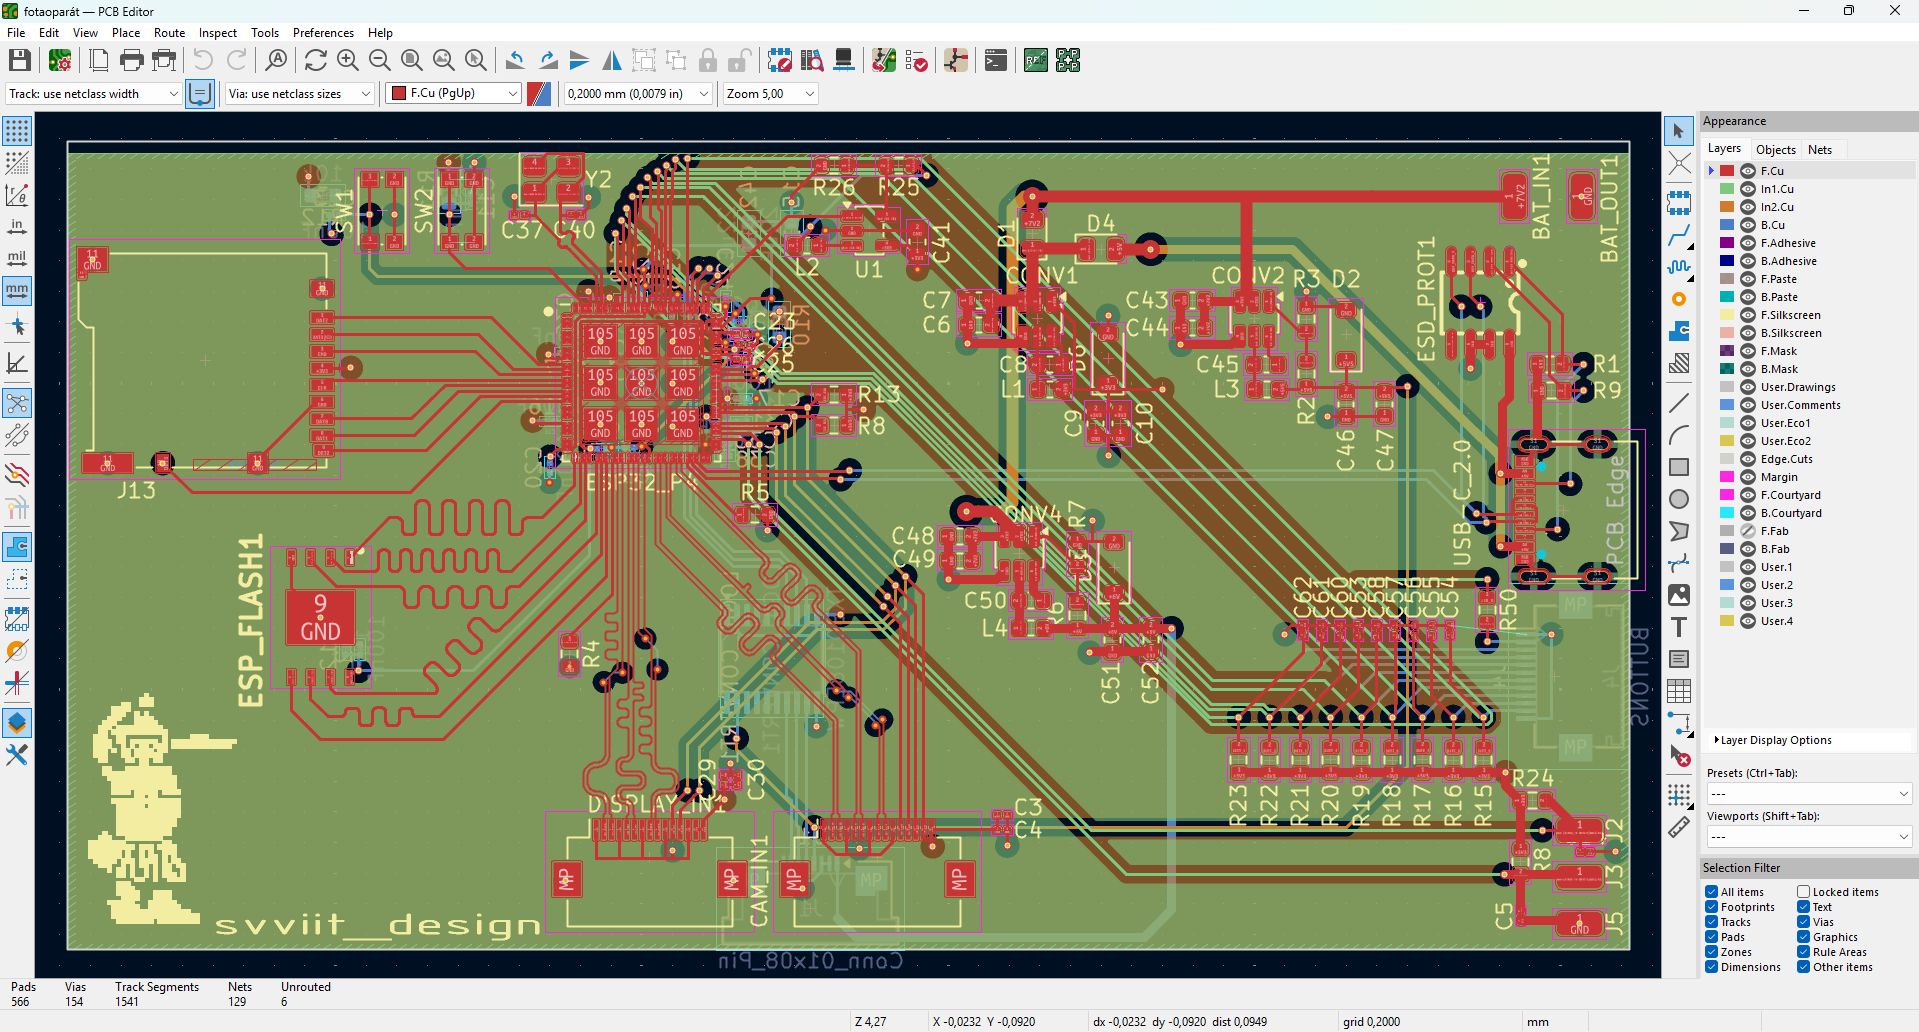
\includegraphics[width=1\linewidth]{pictures/pcbeditor.png}
    \caption{Ukázka programu PCB editor \textit{Zdroj: [vlastní]}}
    \label{fig:pcbsmrdito}
\end{figure}

Jako poslední podstatná část programu KiCAD je gerber veiwer. Ten slouží k exportu geberových dat pro výrobu desky.

\section{Visual Studio Code}
Visual Studio Code (zkráceně VS Code nebo VS) je bezplatné moderní vývojové prostředí. Díky velkému množství rozšíření, která lze instalovat přímo v programu, a podpoře hlavních operačních systémů (Windows, Linux a macOS) si získalo značnou oblibu mezi programátory.

\begin{figure}
    \centering
    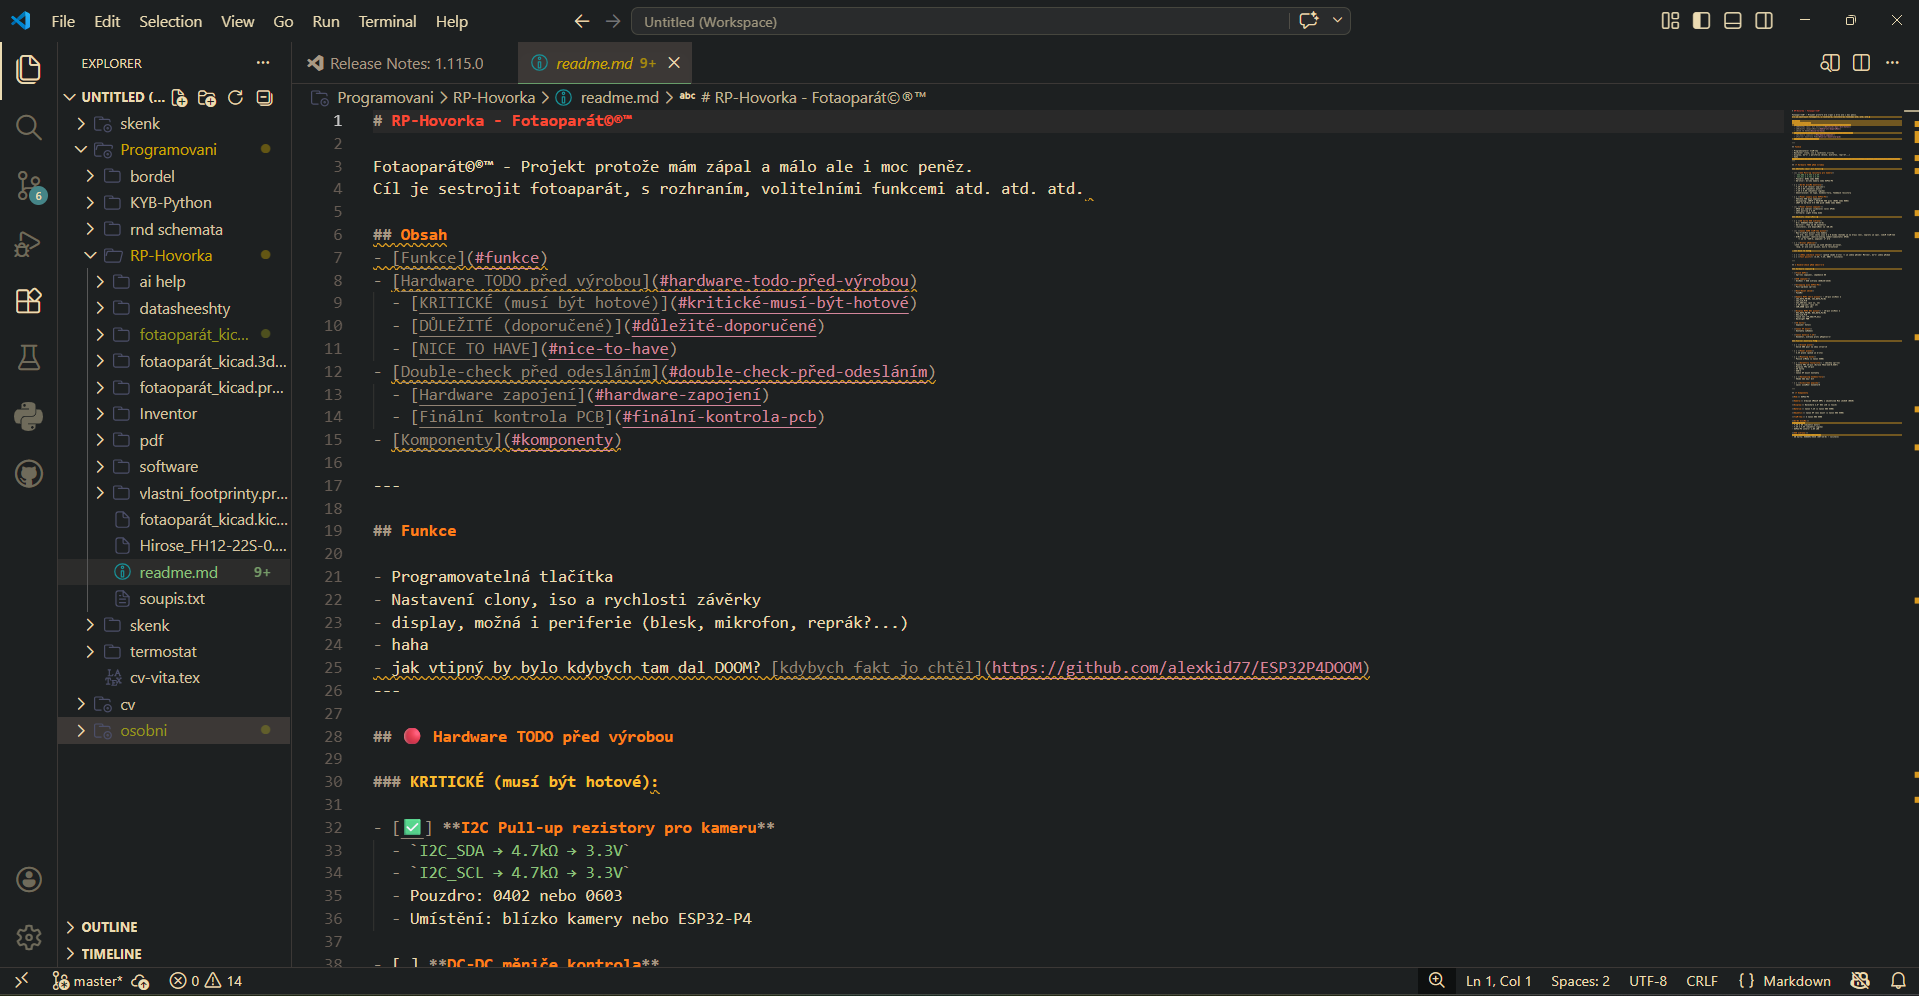
\includegraphics[width=1\linewidth]{pictures/vsko.png}
    \caption{Ukázka programu Visual Studio Code \textit{[Zdroj: Vlastní]}}
    \label{fig:vsko}
\end{figure}

Mezi jeho hlavní funkce patří podpora verzovacích systémů jako např. Git, zvýraznění syntaxe (např. závorkové páry), našeptávání kódu, integrovaný terminál a debugger.

V mé práci jsem VS používal zejména pro jednoduché commitování. Dále jsem v něm používal umělou inteligneci pomocí které jsem napsal část firmwaru. 
\chapter{Vybrané komponenty}
\section{MCU}
Kvůli vysoké výpočetní náročnosti zpracování dat, která představuje jediný snímek o rozlišení 8 Mpx, bylo nutné zvolit jeden z nejvýkonnějších mikrokontrolérů dostupných v době realizace projektu — ESP32-P4. Jedná se o moderní MCU navržené s důrazem na vysoký výpočetní výkon, multimediální zpracování a efektivní práci s periferiemi.

ESP32-P4 je vybaven vícejádrovou architekturou, která umožňuje paralelní zpracování úloh, což je klíčové zejména při práci s obrazovými daty. Dále disponuje hardwarovou akcelerací pro vybrané operace, dostatečnou kapacitou paměti a podporou vysokorychlostních rozhraní, která umožňují efektivní přenos dat z kamerových modulů.

Významnou výhodou této platformy je také široká softwarová podpora a integrace s vývojovým prostředím ESP-IDF, které poskytuje potřebné nástroje pro optimalizaci výkonu a správu systémových prostředků. Díky tomu je možné implementovat i relativně složité algoritmy z oblasti zpracování obrazu přímo na úrovni mikrokontroléru.
\section{Flash paměť}
Další důležitou součástí návrhu je externí flash paměť. Mikrokontrolér ESP32-P4 totiž nedisponuje dostatečně velkou interní pamětí pro uložení uživatelského kódu, a proto je nutné využít externí úložiště.

V tomto projektu byla zvolena paměť W25Q256JV-DTR od společnosti Winbond. Jedná se o sériovou NOR flash paměť s kapacitou 256 Mbit (32 MB), která slouží pro ukládání firmwaru, konfiguračních dat a případně i dočasných obrazových dat.

Paměť komunikuje s mikrokontrolérem prostřednictvím rozhraní SPI, respektive jeho rozšířené varianty QSPI, která umožňuje paralelní přenos dat po více datových linkách. Díky tomu lze dosáhnout výrazně vyšších přenosových rychlostí oproti standardnímu SPI, což je zásadní zejména při práci s většími objemy dat, například obrazovými snímky.

Označení DTR (Double Transfer Rate) znamená, že data jsou přenášena na obou hranách hodinového signálu, čímž dochází k efektivnímu zdvojnásobení propustnosti bez nutnosti zvyšování pracovní frekvence. Tato vlastnost přispívá ke zvýšení celkového výkonu systému při čtení i zápisu dat.

Paměť je organizována do sektorů, což umožňuje efektivní mazání a zápis po blocích. Zároveň podporuje mechanismy ochrany vybraných oblastí proti zápisu, což je výhodné například pro zabezpečení kritických částí firmwaru.

Díky své kapacitě a rychlosti představuje tato paměť vhodné řešení pro aplikace, kde interní paměť mikrokontroléru nepostačuje a kde je nutné pracovat s větším objemem dat při zachování relativně vysoké přenosové rychlosti.
\section{Kamerový modul}
Další klíčovou komponentou je kamerový modul Arducam IMX219 s rozlišením 8 Mpx. Tento modul byl zvolen nejen s ohledem na příznivý poměr ceny a výkonu, ale také díky své kompatibilitě a vhodnosti pro použití s mikrokontrolérem ESP32-P4.

ESP32-P4 disponuje rozhraním DSI/CSI, které umožňuje vysokorychlostní přenos obrazových dat mezi kamerovým modulem, případně displejem, a samotným mikrokontrolérem. Využití tohoto rozhraní je zásadní zejména při práci s obrazem ve vyšším rozlišení, kde by standardní paralelní nebo sériová rozhraní představovala významné omezení.

Samotný snímač IMX219 nabízí dostatečné rozlišení pro zamýšlenou aplikaci a zároveň podporuje různé režimy výstupu, což umožňuje optimalizovat kompromis mezi kvalitou obrazu a objemem přenášených dat. Díky tomu lze přizpůsobit parametry snímání aktuálním výpočetním možnostem systému.

Výhodou modulu Arducam je také jeho široká podpora a dostupná dokumentace, což usnadňuje jeho integraci do návrhu jak na hardwarové, tak i softwarové úrovni. Modul komunikuje prostřednictvím standardizovaného rozhraní, což zjednodušuje jeho zapojení i konfiguraci.

\section{Display}
Pro zobrazovací jednotku jsem zvolil 2,8palcový LCD modul od společnosti Waveshare, a to především díky jeho DSI rozhraní, které je podporováno mikrokontrolérem ESP32-P4. Toto rozhraní umožňuje efektivní a rychlou komunikaci mezi řídicí jednotkou a displejem.

Dalším důvodem výběru tohoto konkrétního displeje byla jeho kompatibilita s mechanickou konstrukcí zařízení. Pro zjednodušení návrhu jsem se rozhodl využít tělo fotoaparátu Canon 550D. Pro účely této kapitoly postačí uvést, že původní displej z modelu 550D není vhodné použít, jelikož k němu není veřejně dostupná dostatečná technická dokumentace. Zároveň má však velmi podobné rozměry jako zvolený Waveshare modul, což usnadňuje jeho náhradu bez nutnosti zásadních mechanických úprav.

\section{Konektor pro SD kartu}

Pro ukládání dat bude použit konektor pro SD kartu, což představuje standardní řešení úložiště u digitálních fotoaparátů. SD karty jsou kompaktní, široce rozšířené a snadno dostupné externí médium, které nabízí dostatečné přenosové rychlosti pro zamýšlenou aplikaci. Oproti tomu běžné USB flash disky nejsou pro tento typ zařízení tak vhodné, a to jak z hlediska rozměrů, tak i způsobu připojení.

Alternativou by mohlo být použití paměťových karet typu CompactFlash. Tyto karty sice teoreticky dosahují vyšších přenosových rychlostí, mimo jiné díky většímu počtu pinů, avšak jejich nevýhodou je vyšší pořizovací cena. Dalším omezením je skutečnost, že konektory pro CompactFlash karty jsou v současnosti obtížně dostupné a často vyžadují použití redukce. Z těchto důvodů nebylo toto řešení dále uvažováno.
\section{Konektor pro komunikaci s počítačem.}
Pro nahrávání firmwaru je na desce navržen USB-C konektor, který slouží nejen pro samotné programování mikrokontroléru, ale také pro jeho napájení během vývoje a testování. Toto řešení výrazně zjednodušuje proces nasazení firmwaru, protože není nutné využívat externí programátor.

Rozhraní USB je implementováno s ohledem na maximální kompatibilitu s běžně dostupnými nástroji a vývojovými prostředími. Díky tomu je možné firmware nahrávat přímo z vývojového prostředí prostřednictvím standardního USB připojení, což urychluje celý vývojový cyklus.
\chapter{Podrobné zapojení na desce}
\section{MCU}
Středem celého návrhu je mikrokontrolér ESP32-P4, osazený jako hlavní výpočetní a řídicí prvek. V zapojení jsou využity jeho vysokorychlostní periferie (MIPI CSI/DSI, USB a rozhraní pro externí flash), zatímco běžné vstupy a výstupy obsluhují ovládací prvky a pomocné funkce.
\begin{figure}
    \centering
    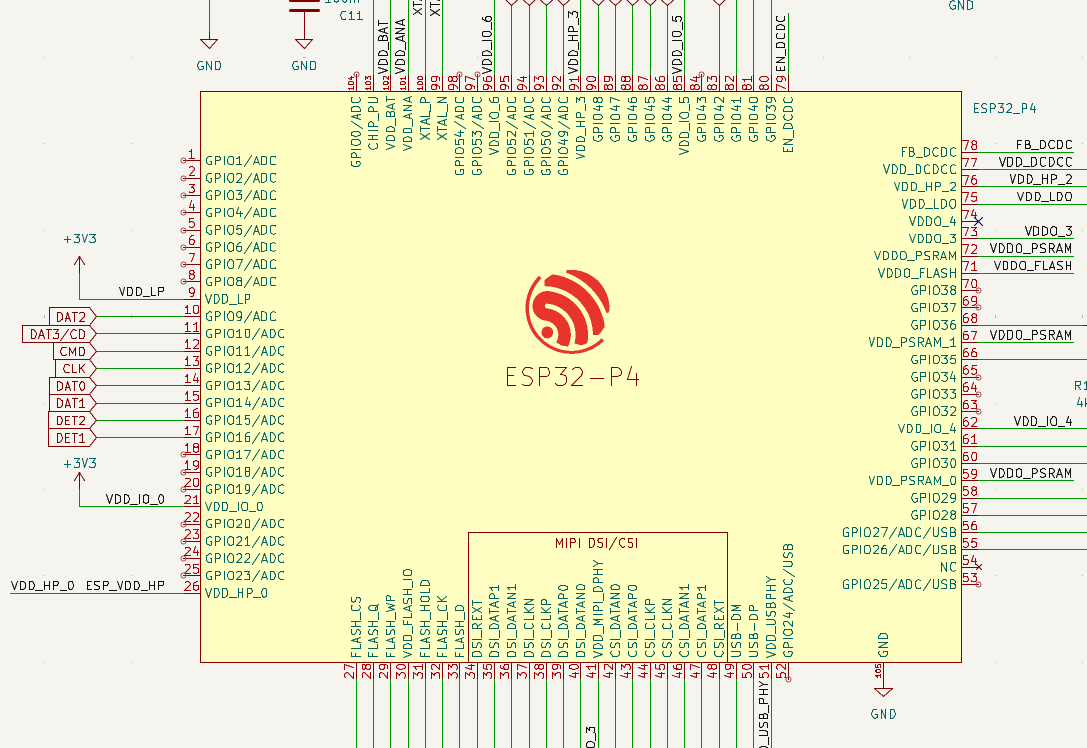
\includegraphics[width=0.7\linewidth]{pictures/esp32-p4.png}
    \caption{ESP32-P4 v eschématu \textit{[Zdroj: Vlastní]}}
    \label{fig:esp32p4}
\end{figure} 
Sám o sobě ale být použit nemůže. Pro jeho ideální funkci je potřeba externí flash pamět, externí krystal a externí buck converter na (doplinit voltage) pro napájení high power pinů. 

Programování zařízení je v tomto projektu navrženo pouze přes USB. Mikrokontrolér sice obecně umožňuje i programování přes UART, tato možnost však v daném návrhu není využita.

Podrobnější informace o doporučeném zapojení napájecích domén a startovacích podmínkách uvádí datasheet a technický referenční manuál výrobce.


\section{Napájení periférií}
Napájecí část je navržena pro provoz z jednoho akumulátoru 7,2 V a je rozdělena do několika samostatných větví podle typu zátěže\cite{local_readme}. Ve schématu jsou osazeny měniče CONV1 (AP63203WU, pevný výstup 3,3 V), CONV2 (AP63200WU) a CONV4 (AP63200WU)\cite{ap63200,local_kicad}.

U měniče CONV1 je osazena výkonová tlumivka L1 (3,9 $\mu$H), vstupní a výstupní filtrační kondenzátory C7 (10 $\mu$F), C10 (22 $\mu$F), C44 (10 $\mu$F), C46 (22 $\mu$F), C48 (100 nF) a C52 (22 $\mu$F), dále ochranná zenerova dioda D6 (3,6 V). USB část je doplněna konfiguračním rezistorem R1 (5,1 k$\Omega$) a ESD ochranou ESDA6V1U1RL\cite{local_kicad,esda6v1,usb_typec}.

U měničů AP63200WU jsou osazeny lokální blokovací a filtrační kondenzátory C16, C17, C19, C21, C22, C32 a C36 (100 nF), dále C25 (1 $\mu$F), C33 (10 $\mu$F) a C34 (10 $\mu$F). V regulační části je použit odporový dělič s R6 (16 k$\Omega$)\cite{local_kicad}. Toto osazení omezuje přenos rušení do citlivých částí systému, zejména kamery, flash paměti a USB.

\section{Externí Flash paměť}
Externí flash paměť je osazena jako samostatný nevolatilní prostor pro firmware a provozní data\cite{w25q256,local_kicad}. Připojení je řešeno přes QSPI, aby byla zajištěna dostatečná propustnost při startu systému i při běhu aplikace.

Ve schématu je osazena paměť ESP\_FLASH1 typu W25Q256JVEIQ. Stabilitu této části zajišťuje zejména lokální blokování napájení a krátké návratové cesty do země, které minimalizují rušení na hodinové a datových linkách\cite{local_kicad,esp32p4_trm}.

\section{Konektor pro zapojení kamerového modulu}
Kamerový modul je připojen přes 15pinový FFC konektor. Vedeny jsou diferenciální páry MIPI CSI, řídicí sběrnice I2C, napájení a řídicí signály pro zapnutí modulu\cite{local_kicad,esp32p4_ds}.

Z pohledu osazení jsou důležité zejména podpůrné prvky na řídicí sběrnici a napájení: pull-up rezistory R13 (4,7 k$\Omega$) a R11 (10 k$\Omega$), doplněné o lokální filtrační kondenzátory napájecí větve. Právě tyto součástky mají přímý vliv na spolehlivou inicializaci kamery po zapnutí\cite{local_kicad,local_readme}.

Text této části je záměrně veden obecně na úrovni použitého rozhraní a zapojení. Konkrétní parametry obrazového snímače je vždy nutné vztáhnout k reálně osazenému kamerovému modulu.

\section{Konektor pro zapojení displaye}
Displej je připojen přes samostatný 15pinový FFC konektor. Na tomto rozhraní jsou vyvedeny MIPI DSI páry pro obrazová data a pomocné signály pro obsluhu dotykové vrstvy\cite{local_kicad,waveshare}.

Podpůrné osazení zahrnuje především stabilní napájení panelu a dotykového obvodu, lokální blokování a odpovídající připojení řídicích linek. U dotykové části je zásadní správné zapojení I2C komunikace, aby nedocházelo k výpadkům při současné aktivitě displeje a kamerové větve.

\section{Dock pro umístění SD karty}
Pro ukládání snímků je osazen konektor pro MicroSD kartu\cite{local_kicad}. Kromě datových linek je využita i detekce vložení karty, což zjednodušuje obsluhu v softwaru a snižuje riziko zápisu na neosazené médium.

V okolí tohoto konektoru jsou důležité ochranné a podpůrné prvky: ESD ochrana datových linek, filtrace napájení karty a krátké návratové cesty do země\cite{esda6v1}. Protože jde o často připojované uživatelské rozhraní, je tato část klíčová pro dlouhodobou spolehlivost zařízení.

\section{Externí krystal}
Hodinový systém je doplněn externím 40MHz krystalem a dvojicí zátěžových kondenzátorů podle doporučení výrobce\cite{local_kicad,esp32p4_ds}. Tato část má přímý vliv na stabilní start systému i na přesnost časování vysokorychlostních periferií.

Z hlediska osazení i návrhu je důležité držet krystal i jeho pasivní síť co nejblíže mikrokontroléru, použít krátké propoje a neprotahovat v okolí rušivé datové linky\cite{esp32p4_trm}.

\section{Převodník logických úrovní pro komunikaci s objektivem}
Pro komunikaci s objektivem Canon EF je osazen obousměrný převodník logických úrovní TXS0108EPW\cite{txs0108e,canon_ef_notes}. Důvodem je rozdíl mezi logikou mikrokontroléru a úrovněmi na straně objektivu.

Podpůrné součástky v této části zahrnují zejména správné napájení obou domén převodníku, blokovací kondenzátory C53 až C56 a C60 až C61 (100 nF) a korektní aktivaci pinu OE přes rezistor R8 (10 k$\Omega$). Bez těchto prvků může být komunikace nestabilní i při správné implementaci protokolu ve firmwaru\cite{local_kicad}.

Z dostupných měření vyplývá, že část EF signálů není spolehlivá při 3,3V úrovni, proto je oddělení napěťových domén v této části nezbytné\cite{canon_ef_notes,magic_lantern}.

\section{Napájení interní SRAM paměti}
Napájení interních paměťových a pomocných bloků MCU je řešeno jako samostatně filtrované části v rámci celkové napájecí topologie čipu\cite{local_kicad,esp32p4_trm}. Cílem je omezit průnik rušení mezi výpočetní částí, vysokorychlostními periferiemi a interními paměťmi.

V praxi to znamená důsledné osazení blokovacích kondenzátorů v bezprostřední blízkosti napájecích pinů a kvalitní zemní návrat. Nedostatečné osazení této podpůrné části se obvykle projeví náhodnými chybami při startu systému, výpadky komunikace nebo nestabilitou při vyšší zátěži\cite{esp32p4_ds}.

\section{USB-C USB 2.0 konektor}
Datové a servisní rozhraní je řešeno přes USB-C v režimu USB 2.0\cite{local_kicad,usb_typec}. Rozhraní je použito pro programování firmware, ladění i napájení během vývoje.

Podpůrné osazení USB části je zásadní: správné zapojení konfiguračních pinů konektoru, ESD ochrana datových linek a kvalitní lokální blokování napájení\cite{esda6v1}. Právě tyto prvky rozhodují o odolnosti proti výbojům při připojování kabelu a o stabilitě komunikace.

V kombinaci s nativní podporou USB v ESP32-P4 toto řešení výrazně zjednodušuje oživení i další vývoj\cite{esp32p4_ds,esp32p4_web}.

\chapter{Plánované oživení}
\chapter{Plánovaná konstrukce}



% CIATCE ---------------------------------------------------------------------------
\begin{thebibliography}{99}
\addcontentsline{toc}{chapter}{Literatura}

% \bibiintem{reference} referenci pak pouzijte v textu \cite{reference}.
% dodržujte formátování citací dle normy: Jméno, název (kurzívou), vydavatel, rok, ...
% Pořadí citací podle výskytu v textu. 

\bibitem{ap63200} DIODES INCORPORATED. \textit{AP63200/AP63201/AP63203/AP63205 -- Buck Converter Datasheet}. Dostupné z: \url{https://www.diodes.com/assets/Datasheets/AP63200-AP63201-AP63203-AP63205.pdf}. [cit. 2026-04-23].

\bibitem{local_kicad} HOVORKA, V. \textit{Projektové schéma v KiCadu (fotaoparát.kicad\_sch, power.kicad\_sch, peripherals.kicad\_sch)}. Lokální projektová dokumentace, 2026.

\bibitem{local_readme} HOVORKA, V. \textit{RP-Hovorka/readme.md -- hardware TODO a napájecí větve}. Lokální projektová dokumentace, 2026.

\bibitem{esp32p4_ds} ESPRESSIF SYSTEMS. \textit{ESP32-P4 Datasheet}. Lokální soubor: datasheeshty/Esp32-p4\_datasheet\_en.pdf, 2026.

\bibitem{esp32p4_trm} ESPRESSIF SYSTEMS. \textit{ESP32-P4 Technical Reference Manual}. Lokální soubor: datasheeshty/Esp32-p4\_technical\_reference\_manual\_en.pdf, 2026.

\bibitem{w25q256} WINBOND. \textit{W25Q256JV -- Serial NOR Flash Datasheet}. Lokální soubor: datasheeshty/w25q256jv dtr revc 10252016.pdf, 2016.

\bibitem{arducam_shop} RPI SHOP CZ. \textit{Arducam IMX219 8 MPx kamerový modul}. Dostupné z: \url{https://rpishop.cz/635962/arducam-imx219-8-mpx-kamerovy-modul-s-objektivem-m12-ls1820-noir/}. [cit. 2026-04-23].

\bibitem{waveshare} WAVESHARE. \textit{2.8inch DSI LCD -- Product Page}. Dostupné z: \url{https://www.waveshare.com/product/displays/2.8inch-dsi-lcd.htm}. [cit. 2026-04-23].

\bibitem{waveshare_wiki} WAVESHARE. \textit{2.8inch\_DSI\_LCD -- Wiki}. Dostupné z: \url{https://www.waveshare.com/wiki/2.8inch_DSI_LCD}. [cit. 2026-04-23].

\bibitem{hirose_dm3} HIROSE ELECTRIC. \textit{DM3 Series -- MicroSD Card Connector Catalog}. Dostupné z: \url{https://www.hirose.com/en/product/document?clcode=&productname=&series=DM3&documenttype=Catalog&lang=en&documentid=D49662_en}. [cit. 2026-04-23].

\bibitem{esda6v1} STMICROELECTRONICS. \textit{ESDA6V1U1RL -- ESD Protection Device}. Dostupné z: \url{https://lcsc.com/product-detail/Diodes-ESD_STMicroelectronics_ESDA6V1U1RL_ESDA6V1U1RL_C118278.html}. [cit. 2026-04-23].

\bibitem{txs0108e} TEXAS INSTRUMENTS. \textit{TXS0108E -- 8-Bit Bidirectional Voltage-Level Translator}. Dostupné z: \url{https://www.ti.com/lit/ds/symlink/txs0108e.pdf}. [cit. 2026-04-23].

\bibitem{canon_ef_notes} HOVORKA, V. \textit{software/canon-ef-protocol-notes.md}. Lokální projektová poznámka (reverse engineering EF sběrnice), 2026.

\bibitem{magic_lantern} MAGIC LANTERN TEAM. \textit{Magic Lantern}. Dostupné z: \url{https://www.magiclantern.fm}. [cit. 2026-04-23].

\bibitem{usb_typec} USB IMPLEMENTERS FORUM. \textit{USB Type-C Specification}. Dostupné z: \url{https://www.usb.org/sites/default/files/documents/usb_type-c.zip}. [cit. 2026-04-23].

\bibitem{esp32p4_web} ESPRESSIF SYSTEMS. \textit{ESP32-P4 Product Overview}. Dostupné z: \url{https://www.espressif.com/en/products/socs/esp32-p4}. [cit. 2026-04-23].


\end{thebibliography}
% konec citací

% Přílohy: 
\chapter*{Přílohy}
\pagenumbering{Roman}
\addcontentsline{toc}{chapter}{Přílohy}



\end{document}